% @Author: AnthonyKenny98
% @Date:   2020-02-28 15:02:19
% @Last Modified by:   AnthonyKenny98
% @Last Modified time: 2020-04-06 13:35:38

Having implemented a functioning version of \gls{RRT} that adhered to the specifications set out in Table \ref{table:RRT_Tech_Specs_Abbrev}, analysis of its computational profile could begin. The purpose of this analysis is to identify the biggest bottleneck of \gls{RRT} and therefore the best opportunity for hardware acceleration.

\subsection{Experimental Methodology}
    Experiments were set up to determine which of the 5 key functions of \gls{RRT} takes up the biggest share of computational load. The only fair way of determining computational load of each function is to measure the percentage of \gls{CPU} time each function takes in the \textbf{fastest possible execution} of \gls{RRT} for a given map size. This is explained in more detail in Section \ref{section:rrt_optimal_params}.

    \subsubsection{Measuring Performance}
        The ``performance'' metric of interest is the percentage of total time the \gls{CPU} spends executing each of the 5 aforementioned key functions. CPU analysis of a program can often be more complicated than merely timing how long each function takes to execute. Software can be written with inbuilt multithreading and other optimizations that require special CPU analysis software, such as Intel's VTune Profiler\cite{Intel2019}. This software is designed to find computational bottlenecks in large, complex programs. However, it takes significantly longer to run (which was unsuitable for running hundreds of thousands of tests) and is less customizable than adding performance timers directly to the program's code. It was also hypothesized that, since this project's implementation of \gls{RRT} did not use multithreading or any other timing distorting optimizations, custom performance tracking should yield the same results as VTune Profiler. As such, custom performance tracking was added to the \gls{RRT} implementation. This custom performance tracking method was verified by conducting a $\chi^2$ test against data from VTune Profiler, and was found to be accurate. Appendix \ref{section:rrt_appendix_timing} gives more detail on timing methodology.

    \subsubsection{Optimal Parameters}
    \label{section:rrt_optimal_params}
        Extensive testing was undertaken to determine the optimal parameters for a given map size. The goal was to find the set of parameter values for which \gls{RRT} would reach its goal with $\geq98\%$ probability, for a wide variety of \glspl{OGM}, in the shortest possible time. 

        For each map size ${4, 8, 16, 32, 64}$,the parameters that were varied were $\epsilon$, $K$, and Goal Bias. The success rate and average execution time was measured by, for each set of parameter values, running \gls{RRT} 100 times. Thus, with 5 different map sizes, if 4 values were tested for each parameter, and 4 different \glspl{OGM} were tested, the total number of tests $= 4^4 \times 5 = 1280$ (with each test running \gls{RRT} 100 times!)

        As such, only the optimal parameter values for each map size in included in Table \ref{table:optimal_params}.

        % @Author: AnthonyKenny98
% @Date:   2020-04-06 10:56:43
% @Last Modified by:   AnthonyKenny98
% @Last Modified time: 2020-04-06 11:12:10

\begin{table}[H]
\begin{centering}
\begin{tabular}{|c|c|c|c|c|}
\hline
$DIM$ & $K$ & $\epsilon$ & Goal Bias (\%) & Success Rate (\%) \\
\hline
\hline
\multicolumn{5}{|c|}{2D} \\
\hline
$4\times 4$ & 75 & 1 & 10 & 100 \\
\hline
$8\times 8$ & 100 & 2 & 25 & 98 \\
\hline
$16\times 16$ & 125 & 4 & 25 & 99 \\
\hline
$32\times 32$ & 250 & 8 & 10 & 100 \\
\hline
$64\times 64$ & 500 & 16 & 25 & 100 \\
\hline
\hline
\multicolumn{5}{|c|}{3D} \\
\hline
$4\times 4 \times 4$ & 75 & 1 & 10 & 99 \\
\hline
$8\times 8 \times 8$ & 100 & 2 & 25 & 100 \\
\hline
$16\times 16 \times 16$ & 100 & 4 & 25 & 100 \\
\hline
$32\times 32 \times 32$ & 250 & 8 & 10 & 99 \\
\hline
$64\times 64 \times 64$ & 500 & 16 & 25 & 100 \\
\hline
\end{tabular}
\caption[Optimal RRT Parameters for each Map Size]{\textbf{Optimal RRT Parameters for each Map Size}, shows the optimal set of parameters after extensive testing, alongside their respective success rates over 100 executions of \gls{RRT} for different \glspl{OGM}.}
\label{table:optimal_params}
\end{centering}
\end{table}

\subsection{Results}
\label{section:rrt_analysis_results}
    As expected, the total execution time of \gls{RRT} for optimal parameters increased as the size of the map increased, shown in Figure \ref{fig:rrt_profiling_timing}.

    \begin{figure}[H]
    \begin{centering}
    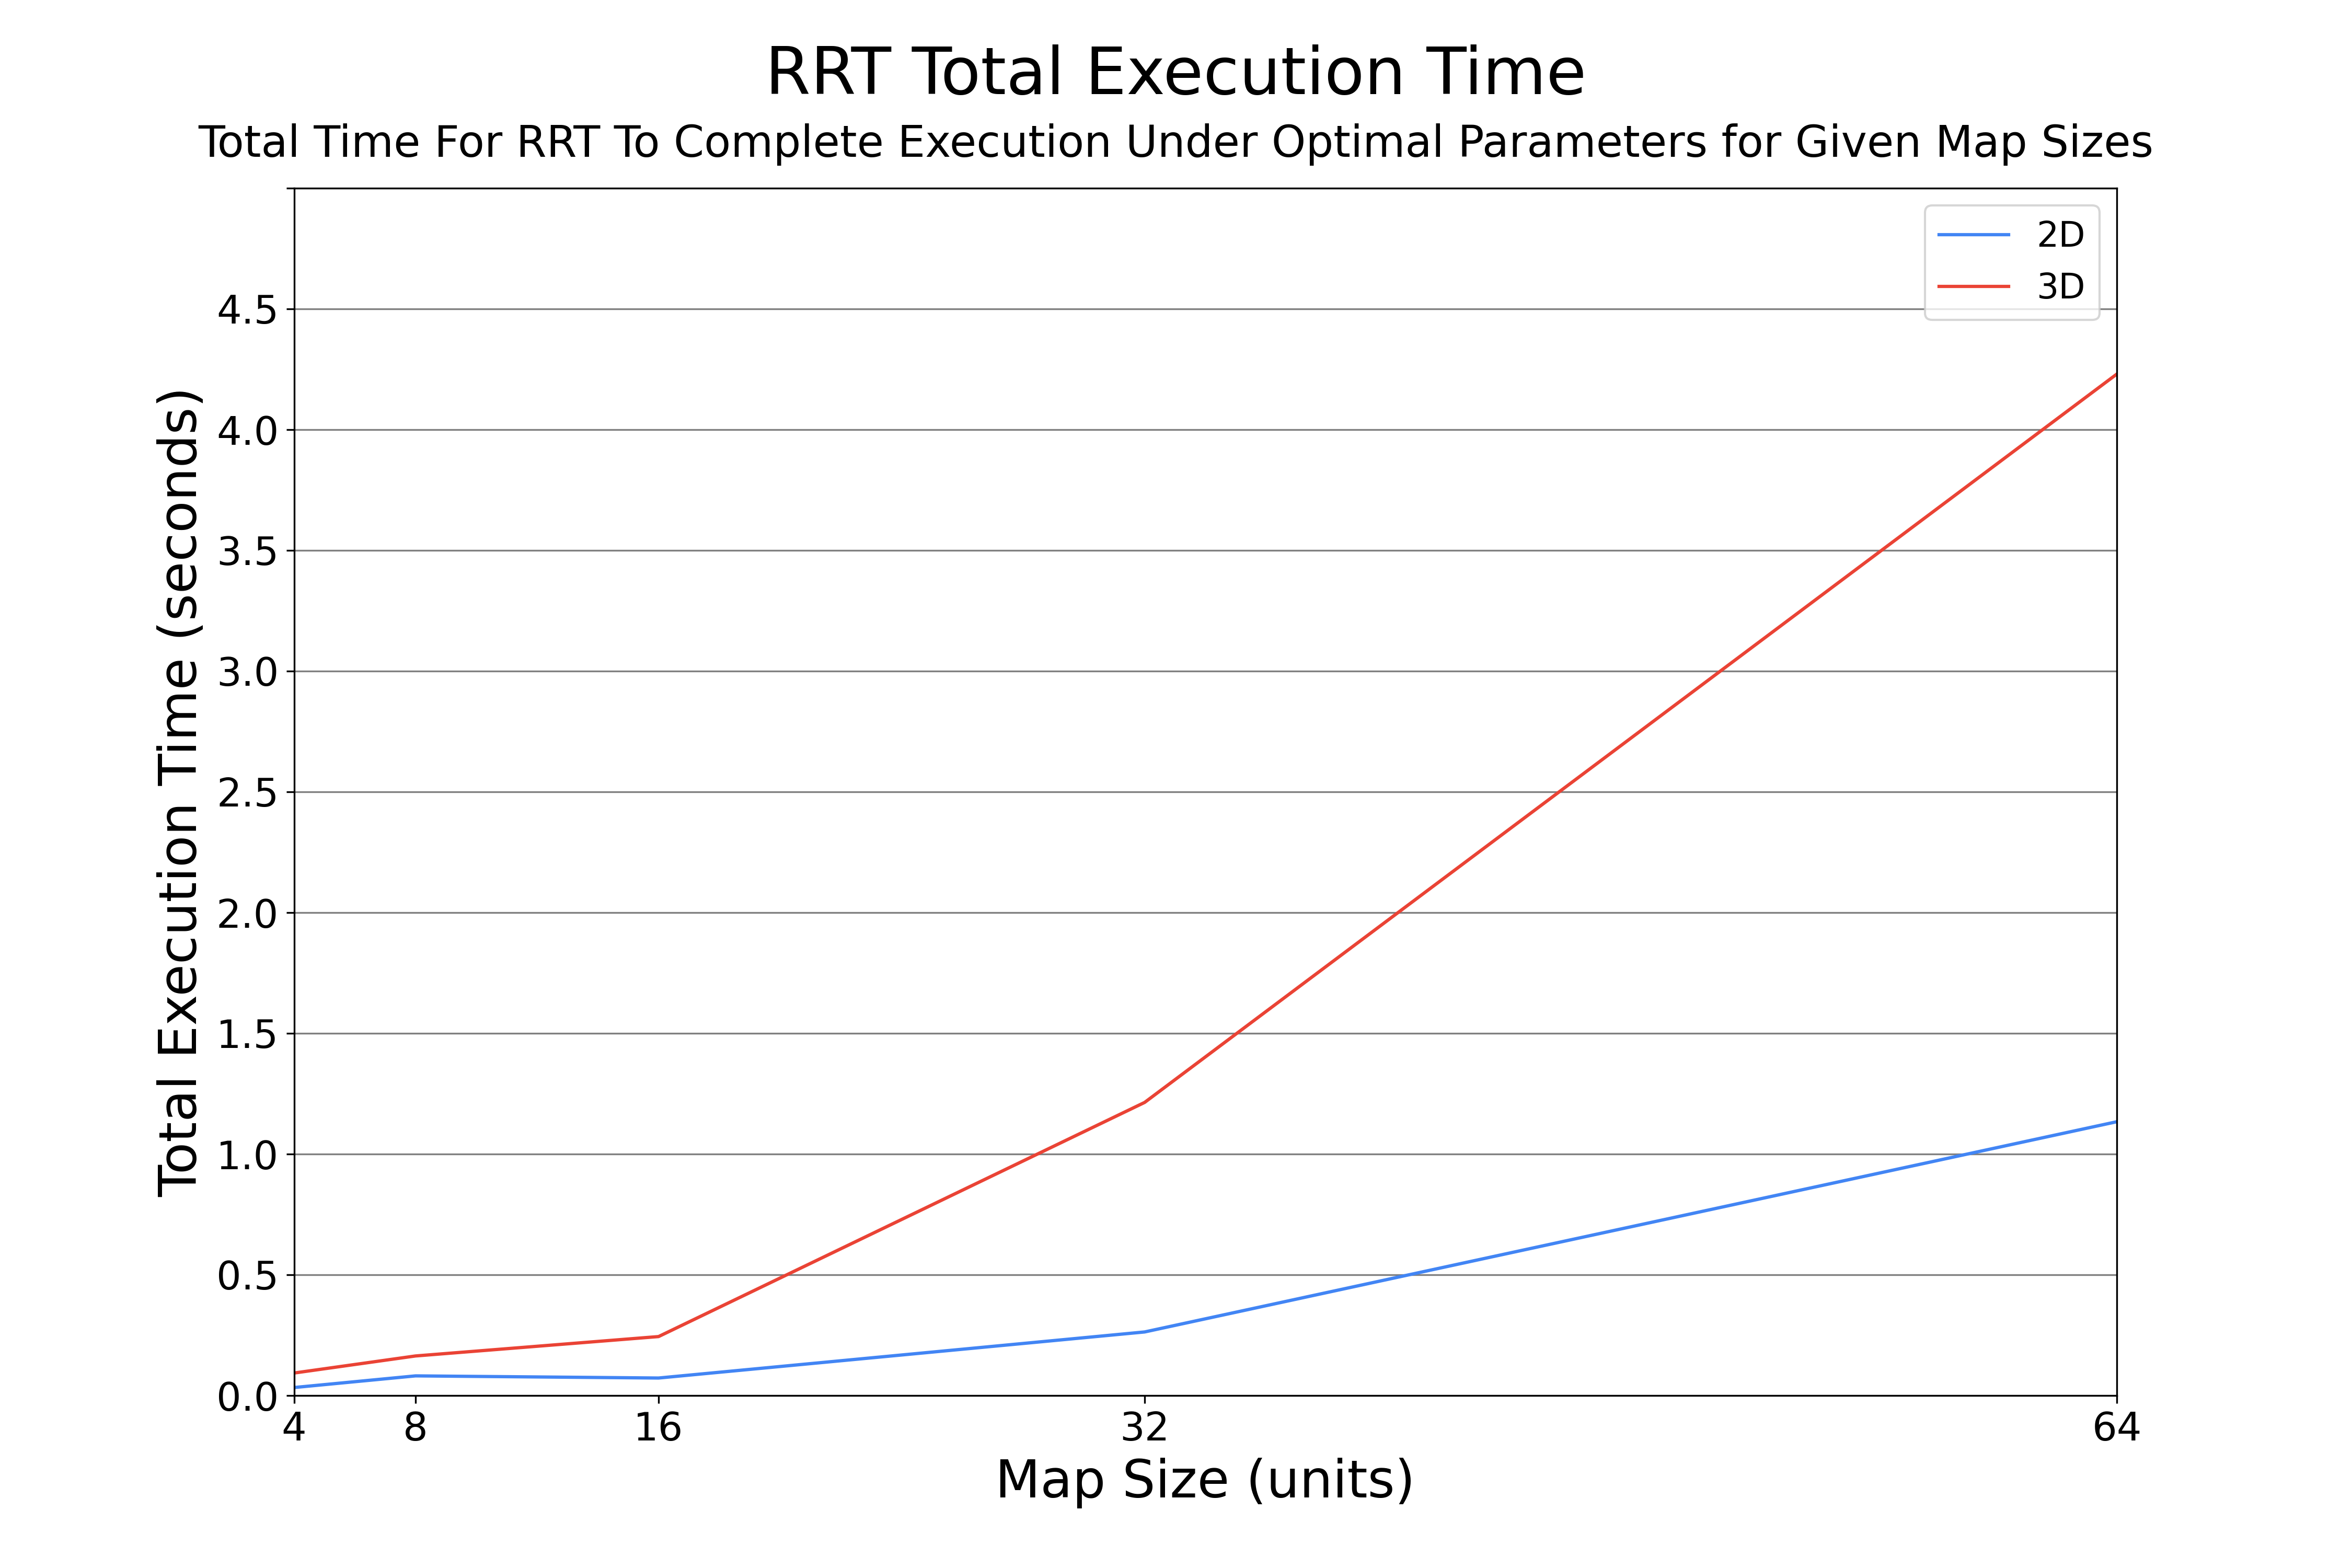
\includegraphics[width=0.65\linewidth]{chapters/chapter2/img/profiling/timing.png}
    \caption[Increasing Total Execution Time of RRT with Map Size]{\textbf{Increasing Total Execution Time of RRT with Map Size}}
    \label{fig:rrt_profiling_timing}
    \end{centering}
    \end{figure}
    
    \subsubsection{2D Computational Load Profile}
        Figure \ref{fig:rrt_profiling_2d} shows that the two biggest computational loads are \texttt{findNearestConfig()} and \texttt{edgeCollisions()}, with the latter increasing as the size of the map increases. The fact that the load of \texttt{edgeCollisions()} and takes the majority of execution in bigger map sizes means that, at least in 2D, it can be considered the bottleneck function.

        % @Author: AnthonyKenny98
% @Date:   2020-02-29 14:51:44
% @Last Modified by:   AnthonyKenny98
% @Last Modified time: 2020-04-06 11:25:12
\begin{figure}[H]
\begin{center}
    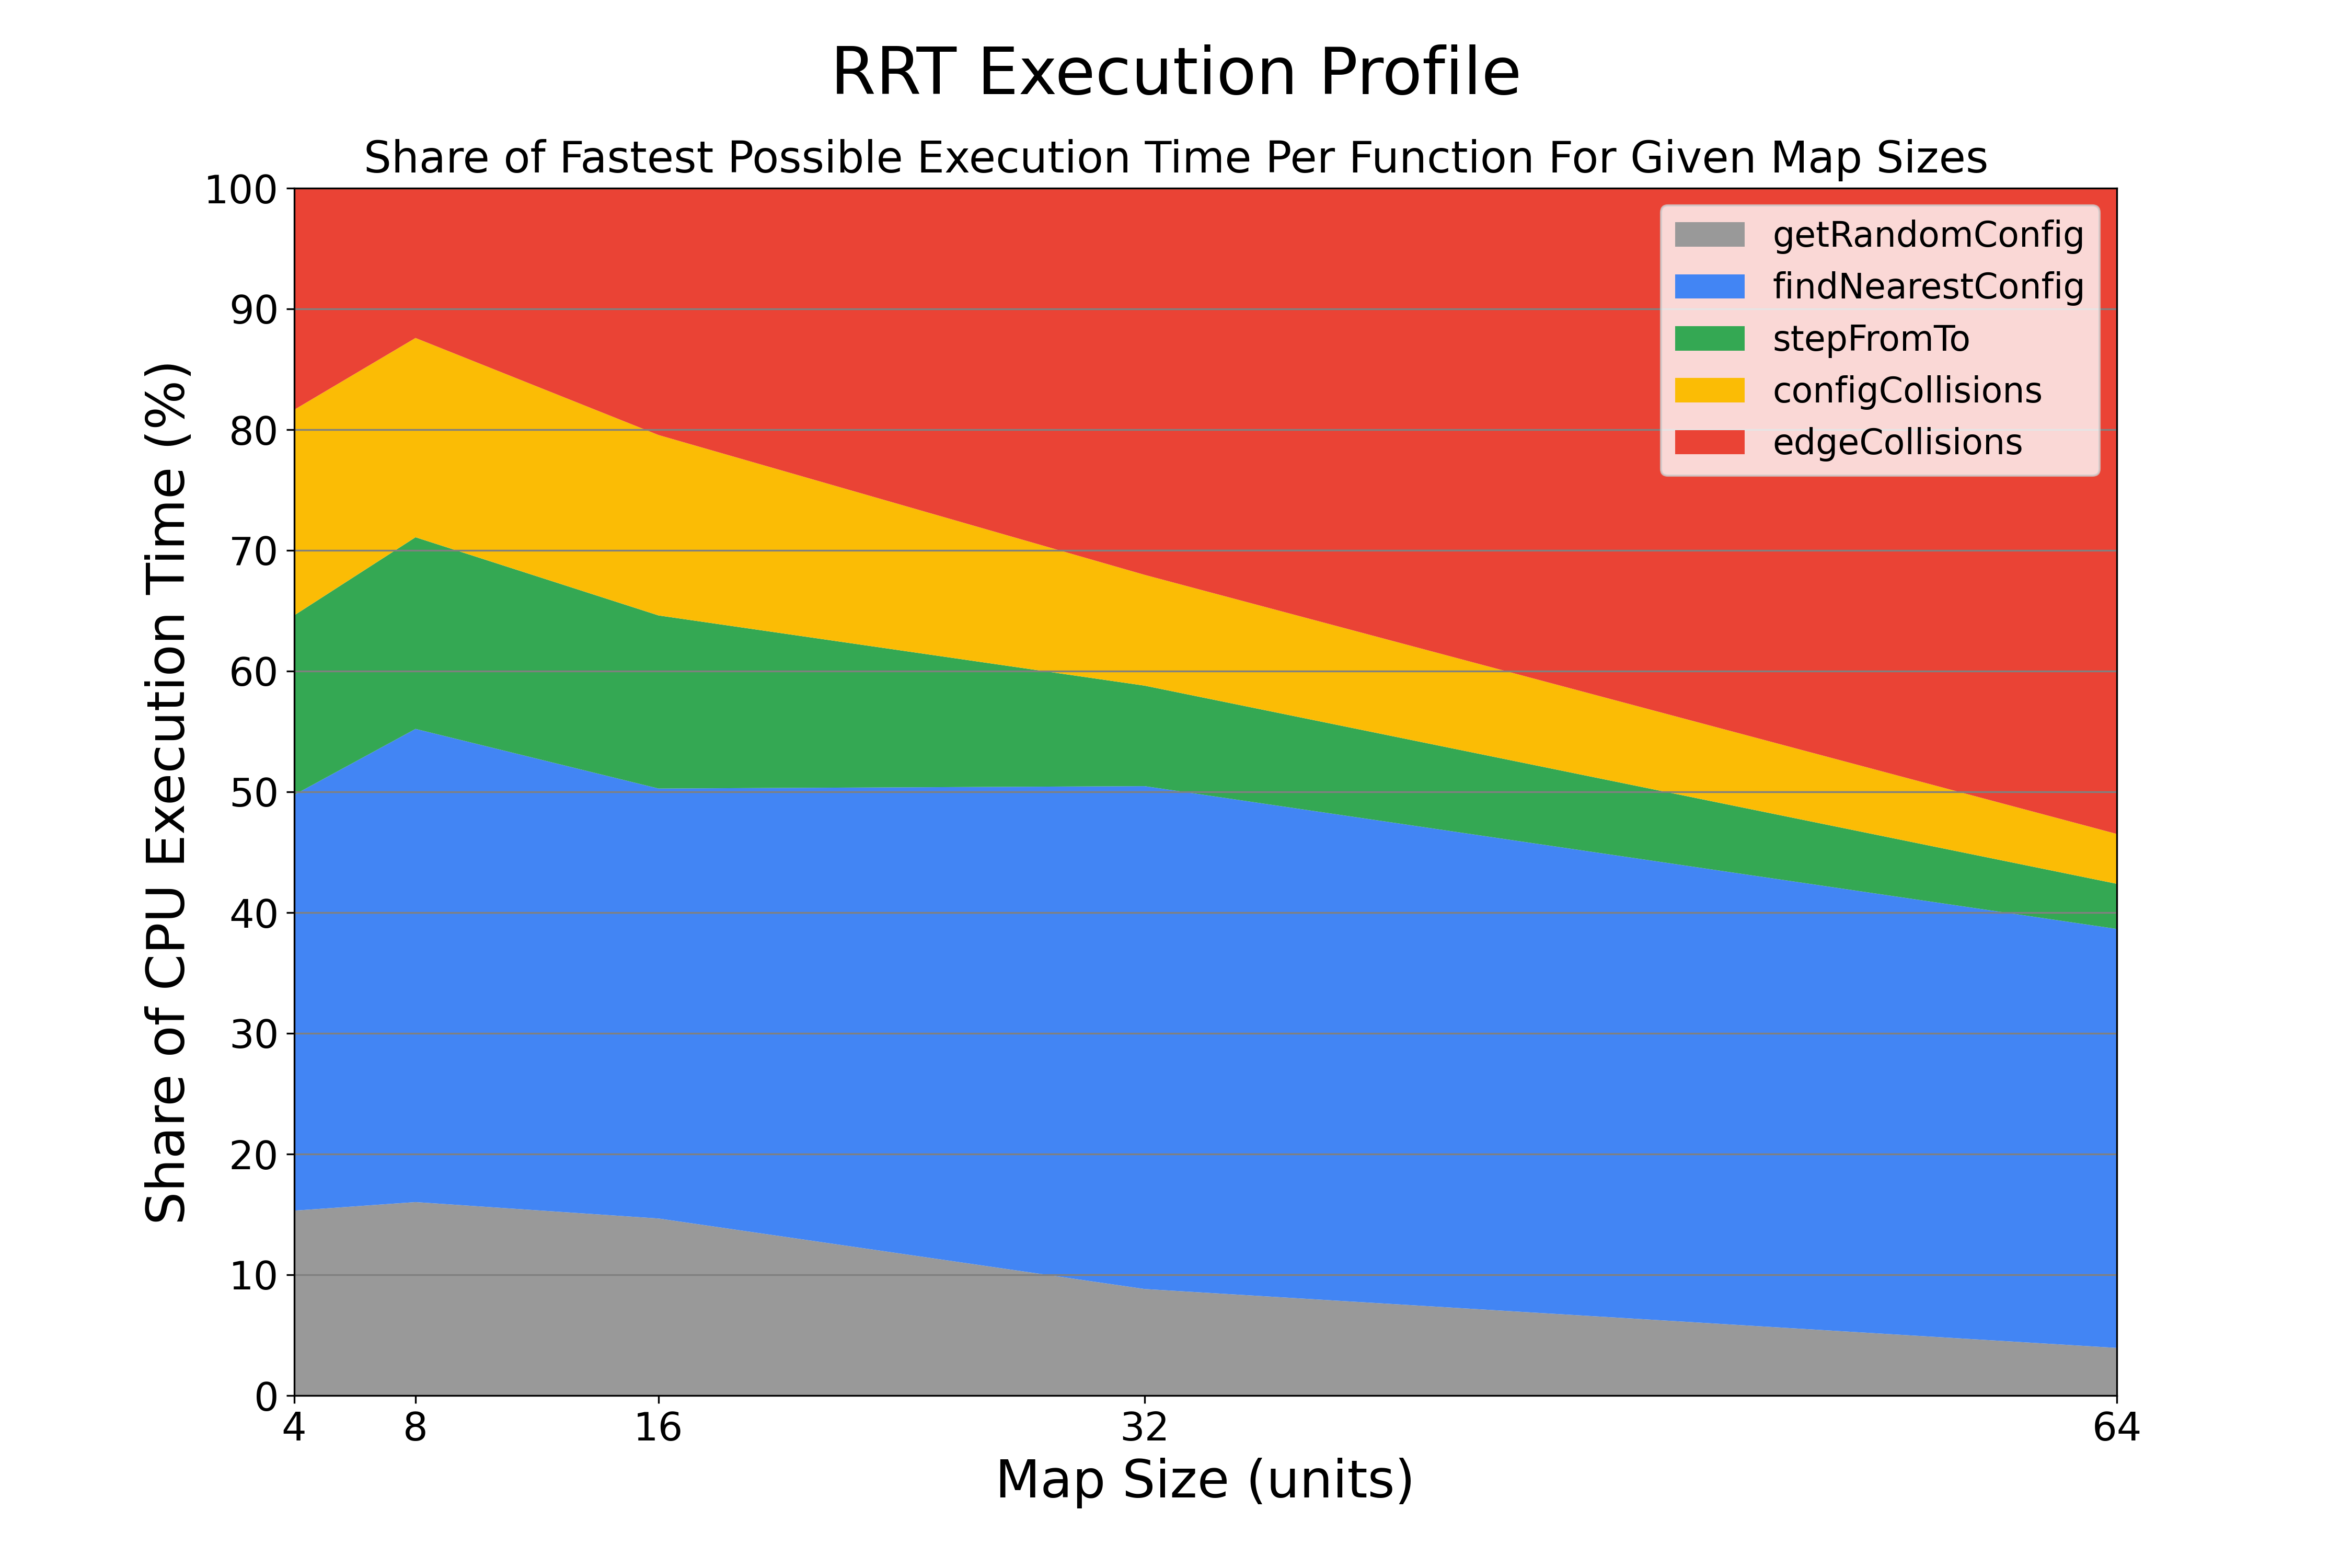
\includegraphics[width=\linewidth]{chapters/chapter2/img/profiling/profile2d.png}
    \caption{Profile of Computational Load of \gls{RRT} in 2D}
    \label{fig:rrt_profiling_2d}
\end{center}
\end{figure}

    \subsubsection{3D Computational Load Profile}
        The computational load of \texttt{edgeCollisions()} was even greater in 3D, starting at 40\% for $4\times 4\times 4$ maps and increasing to 70\% for $64\times 64\times 64$ maps, as shown in Figure \ref{fig:rrt_profiling_3d}.

        % @Author: AnthonyKenny98
% @Date:   2020-02-29 17:30:44
% @Last Modified by:   AnthonyKenny98
% @Last Modified time: 2020-04-06 15:23:45
\begin{figure}[H]
\begin{center}
    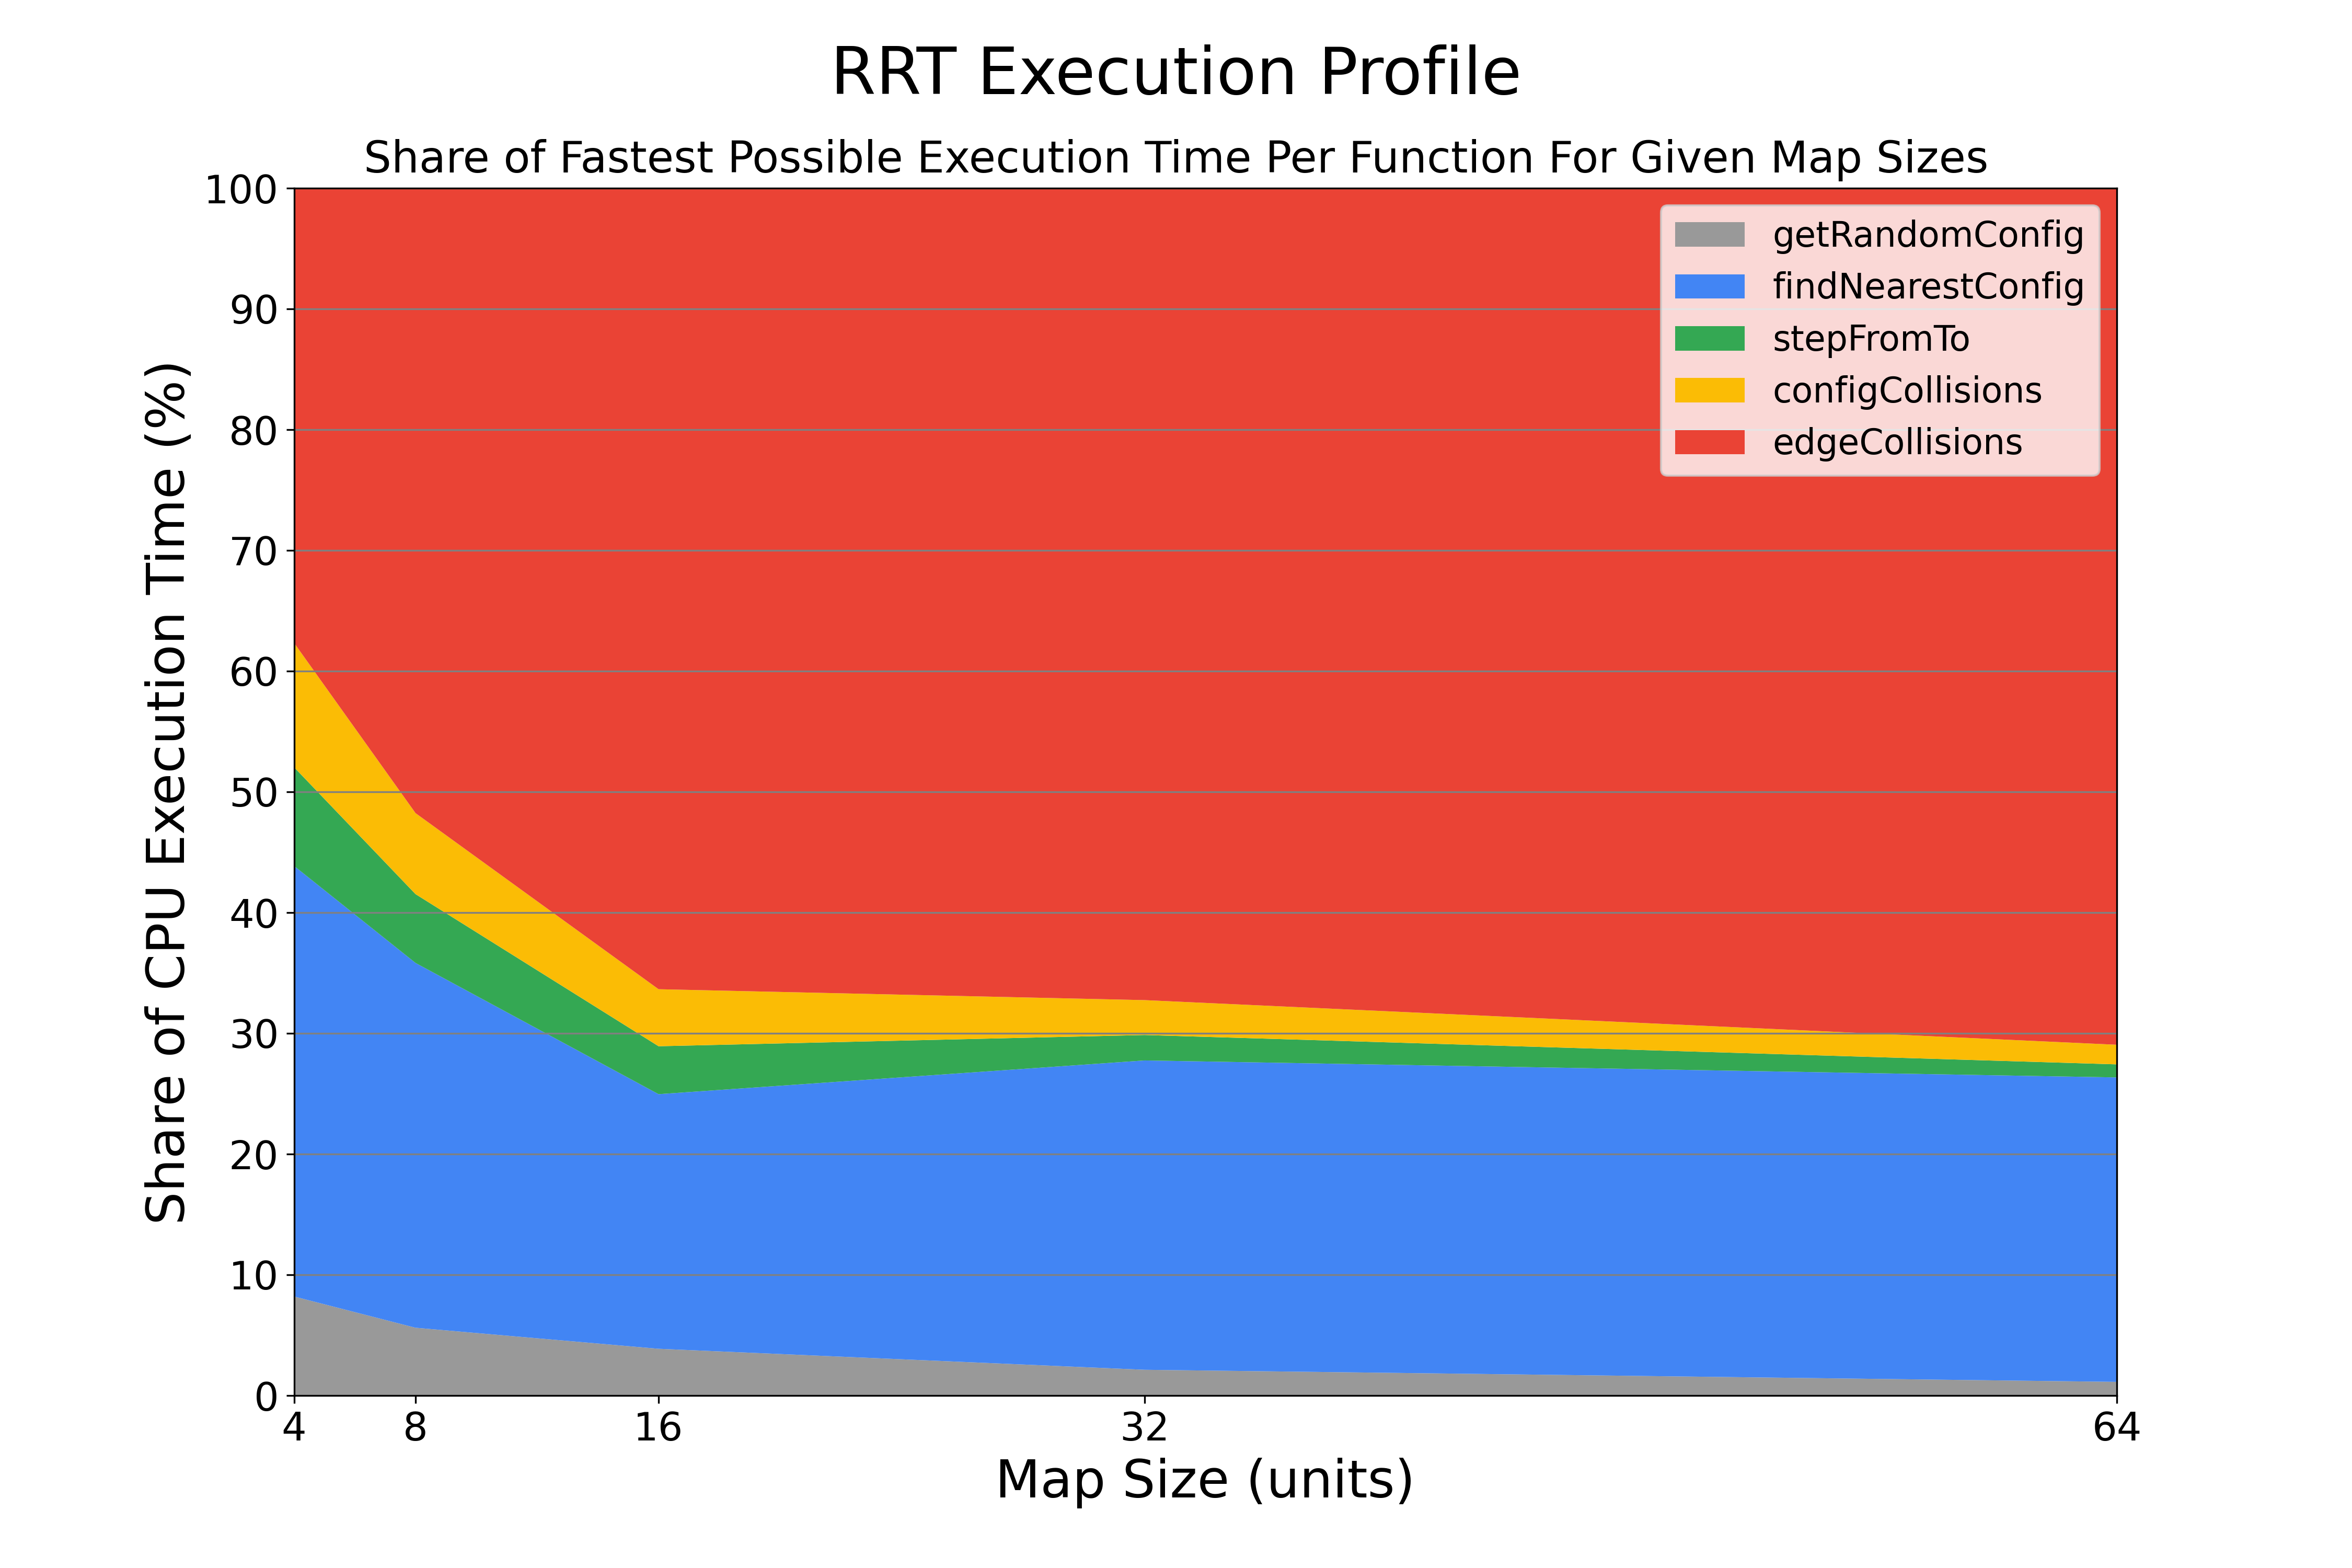
\includegraphics[width=\linewidth]{chapters/chapter2/img/profiling/profile3d.png}
    \mycaption{Profile of Computational Load of \gls{RRT} in 3D}{}
    \label{fig:rrt_profiling_3d}
\end{center}
\end{figure}

        As such, it is safe to say that the bottleneck function for \gls{RRT} is texttt{edgeCollisions()}. This conclusion is strengthened by the fact that \texttt{edgeCollisions()} was implemented in the fastest possible way (without relying on approximations or implementing multithreading), whereas \texttt{findNearestConfig} was implemented without any optimizations (a possibility might have been $K$-nearest nodes). Finally, this conclusion supports prior research that collision detection takes up the vast majority of CPU execution time. As such, this is the function that was targeted for hardware acceleration.  
